%==============================================================================
%== template for LATEX poster =================================================
%==============================================================================
%
%--A0 beamer slide-------------------------------------------------------------
\documentclass[final]{beamer}
\usepackage[orientation=landscape,size=a0,
            scale=1.35         % font scale factor
           ]{beamerposter}
           
\geometry{
  hmargin=2.5cm, % little modification of margins
}

%
\usepackage[utf8]{inputenc}
\usepackage{graphicx}
\linespread{1.15}
%
%==The poster style============================================================
\usetheme{sharelatex}
%==Title, date and authors of the poster=======================================
\title
[BAPG XI, 6 December 2014, Davis, CA, USA] % Conference
{ % Poster title
ANGSD-wrapper: scripts to streamline and visualize NGS population genetics analysis
}

\author{ % Authors
Arun Durvasula\inst{1}, Tyler Kent\inst{1}, Siddharth Bhadra-Lobo\inst{1}, Jeffrey Ross-Ibarra\inst{2}
}
\institute
[University of California, Davis] % General University
{
\inst{1} Dept. of Plant Sciences, University of California Davis\\[0.3ex]
\inst{2} Dept. of Plant Sciences, Center for Population Biology, and Genome Center, University of California Davis\\[0.3ex]
}
\date{\today}
\begin{document}


\begin{frame}[t]
%==============================================================================
\begin{multicols}{3}
%==============================================================================
%==The poster content==========================================================
%==============================================================================

\section{Introduction}

The advent of highly multiplexed sequencing has opened a number of exciting avenues for evolutionary biologists. 
One of the powerful approaches enabled by inexpensive sequencing is the ability to sequence a large number of individuals, each to relatively low sequencing depth. 
However, this approach also presents statistical challenges in the analysis of low coverage data.  
The software ANGSD \cite{Korneliussen} and related programs \cite{Fumagalli} were developed to deal with low coverage sequence data. %Fumagalli 2014 bioinformatics http://www.ncbi.nlm.nih.gov/pubmed/24458950
Rather than call genotypes at variable sites, ANGSD performs a number of population genetic analyses on genotype likelihoods, including estimation of the population mutation rate $\theta$, the site frequency spectrum, neutrality tests, inbreeding coefficients, and population structure.
ANGSD has already been used in several studies to analyze genome sequence data \cite{Crawford} \cite{Lohmueller}. %add cites
However, ANGSD requires considerable familiarity with command line tools and remains inaccessible to many biologists that are not from a computational background. 

Here we present a software package that aids in the preparation of analyses for ANGSD and provides interactive graphing software implemented in R \cite{R} and Shiny \cite{Shiny}.  %add cites
ANGSD-wrapper simplifies multistep analyses such as calculating Tajima’s D into a single step.
Users supply all the needed information in a single configuration file \ref{configfile}, and after ANGSD has finished calculations, ANGSD-wrapper provides interactive graphing of the results \ref{shinygraph}.

\section{Implementation}

ANGSD-wrapper is implemented using bash scripts that call ANGSD methods and handle saving intermediate files between the initial data preparation and the final data analysis. 
Each overall method in ANGSD, such as calculating estimates of $\theta$, follows a specific order of program calls. 
Thus, we have abstracted away the running of each step and provided a set of default values for parameters and instead require the user to supply the data using a configuration file (Figure \ref{configfile}). 
The user can override the default values of the parameters in the configuration file as well.
	
Additionally, ANGSD-wrapper contains a powerful graphing application based on R and Shiny (Figure \ref{shinygraph}). 
After analysis is done by ANGSD, the user can load the resulting statistics into a web-based application hosted on the user’s computer. 
This application allows the interactive plotting of values such as estimators of $\theta$ and Tajima’s D as well as the ability to load gene annotations from Ensembl. 
These features make it easy and intuitive to analyze next generation sequencing data. 

\vskip1ex
\begin{figure}[T!]
  \centering
	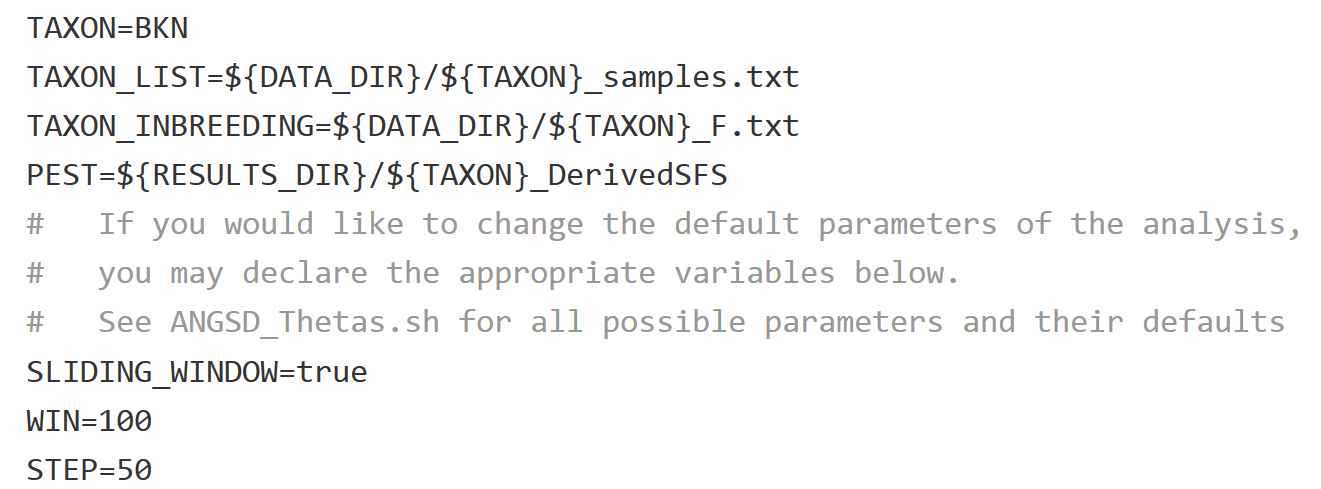
\includegraphics[width=0.75\columnwidth]{conf.png} 
	\caption{Example configuration file}
	\label{configfile}
\end{figure}
  
\begin{figure}[T!]
  \centering
	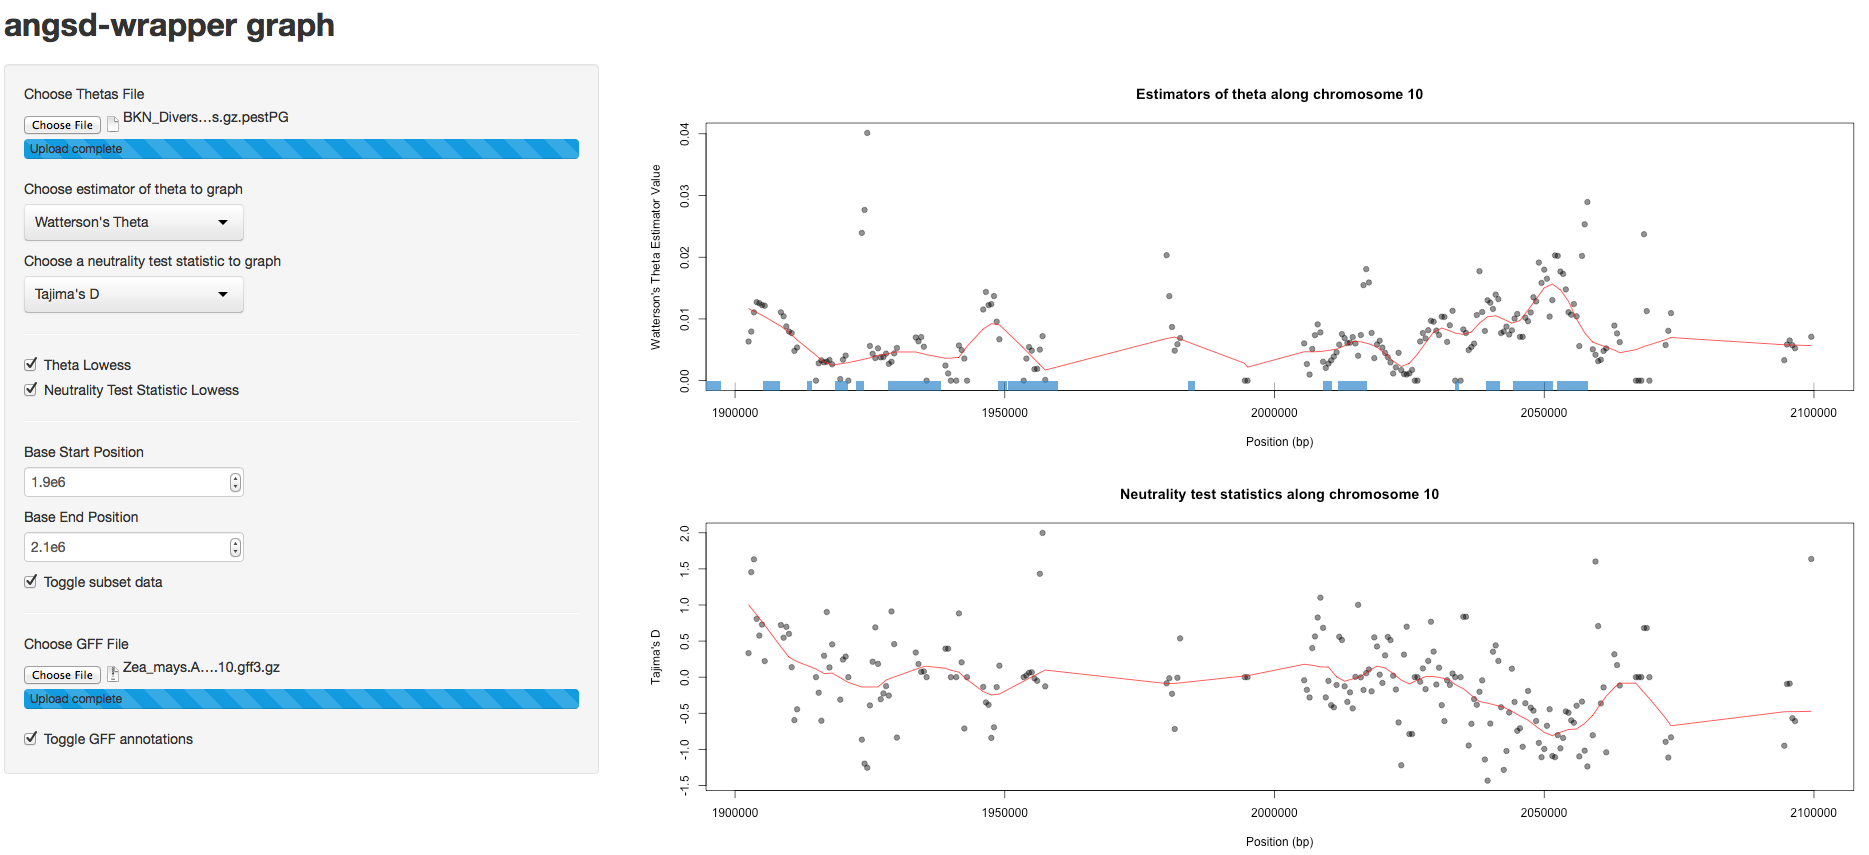
\includegraphics[width=0.99\columnwidth]{screenshot.png}
	\caption{Interactive plotting with Shiny showing a 200kb region along chromosome 10 of \emph{Zea mays}. Blue rectangles are annotated genes.}
	\label{shinygraph}
\end{figure}
\vskip2ex


%        \centering
%        \begin{subfigure}
%				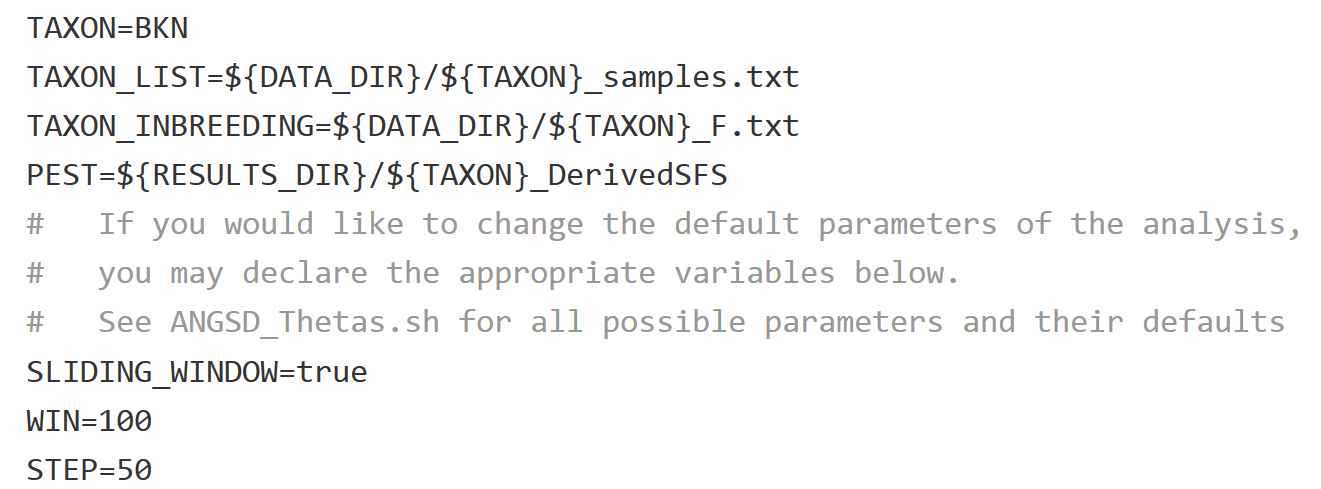
\includegraphics[width=0.75\columnwidth]{conf.png}                
%				%                \label{configfile}
%        \end{subfigure}%
%        ~ %add desired spacing between images, e. g. ~, \quad, \qquad, \hfill etc.
%          %(or a blank line to force the subfigure onto a new line)
%        \begin{subfigure}{0.3\textwidth}
%				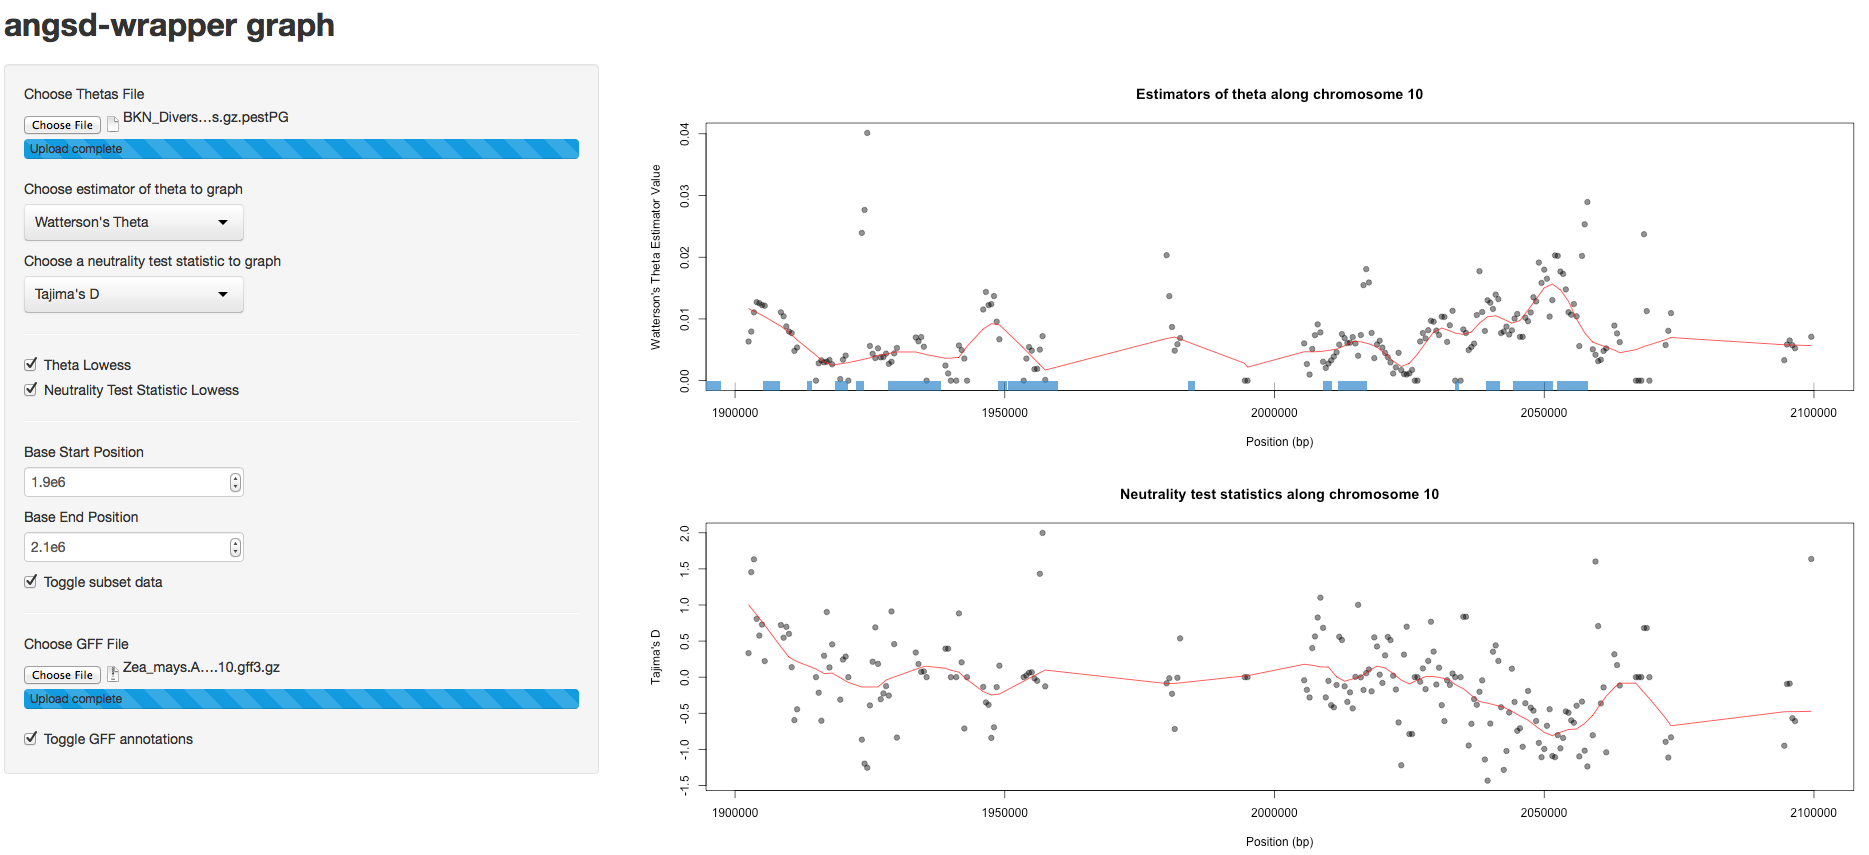
\includegraphics[width=0.99\columnwidth]{screenshot.png}
%                \caption{Interactive plotting with Shiny}
%                \label{shinygraph}
%        \end{subfigure}
%        ~ %add desired spacing between images, e. g. ~, \quad, \qquad, \hfill etc.
%          %(or a blank line to force the subfigure onto a new line)
%         
%		

\section{Example Application}

We sequenced 8 genomes of the wild rice \emph{Oryza glumaepatula}, 4 each from populations allopatric and sympatric to cultivated fields of the domesticated \emph{Oryza sativa} ssp. \emph{indica}, in order to investigate evidence of crop-wild introgression. 
\emph{O. glumaepatula} is a potentially endangered species 1.8 MY diverged from domesticated rice \cite{Zhang} and native to Central and South America \cite{Vaughan}. 
Both species share the AA genome \cite{Vaughan} and we have successfully crossed them experimentally, providing reason to believe the possibility of natural hybridization and thus the risk of wild population decline and extinction \cite{Rhymer}. 
Preliminary analysis using ANGSD-wrapper is suggestive of introgression (Figure \ref{gluma}) as evidenced by the higher correlation of nucleotide diversity ($\pi$) between domesticated rice and the sympatric population (Spearman's $\rho=XXX$) than between domesticated rice and allopatric O. glumaepatula (XXX).

%make this a caption on the figure
\vskip1ex
\begin{figure}
\centering
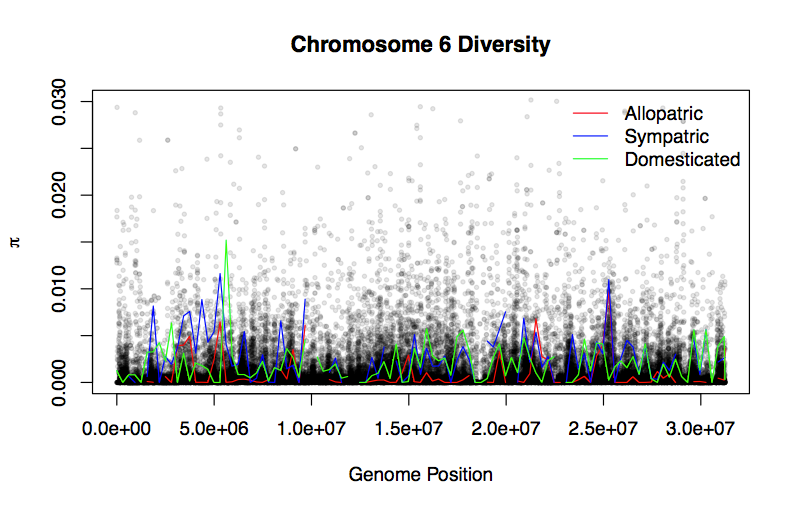
\includegraphics[width=0.99\columnwidth]{chr6rice.png}
\caption{Nucleotide diversity ($\pi$) along chromosome 6 of \emph{Oryza glumaepatula} and \emph{Oryza sativa}}
\label{gluma}
\end{figure}
\vskip2ex




%==============================================================================
%==End of content==============================================================
%==============================================================================

%--References------------------------------------------------------------------

\section{References}

\begin{thebibliography}{99}


%Buso GSG, Rangel PH and Ferreira ME (2001). Mol Ecol 7:107-117.
%Ge S, Oliveira GCX, Schaal BA, Gao LZ and Hong DY (1999) RAPD variation within and between natural populations of the 	wild rice Oryza rufipogan from China and Brazil. Heredity 82:1-7.
%Karasawa, M. M. G., et al. (2007). "Genetic structure of Brazilian wild rice (Oryza glumaepatula Steud., Poaceae) populations 	analyzed using microsatellite markers.” Genetics and Molecular Biology 30: 400-410.
%
%Oka HI (1988) Origin of Cultivated Rice. Japan Scientific Societies Press, Tokyo, and Elsevier Science Publishers, Amsterdam, 	254 pp.
%R Core Team (2014). R: A language and environment for statistical computing. R Foundation for Statistical Computing, 	Vienna, Austria. URL .
%RStudio and Inc. (2014). shiny: Web Application Framework for R. R package version 0.10.2.1. http://CRAN.R-project.org/	package=shiny

\bibitem{Crawford} Crawford, J., M. M. Riehle, W. M. Guelbeogo, A. Gneme, N. f. Sagnon, K. D. Vernick, R. Nielsen and B. P. Lazzaro (2014). Reticulate speciation and adaptive introgression in the Anopheles gambiae species complex.

\bibitem{Fumagalli} Fumagalli, M., F. G. Vieira, T. Linderoth and R. Nielsen (2014). "ngsTools: methods for population genetics analyses from next-generation sequencing data." Bioinformatics 30(10): 1486-1487.

\bibitem{Korneliussen} Korneliussen et al. (2014). BMC Bioinformatics. 15:356

\bibitem{Lohmueller} Lohmueller, K. E., Sparsø, T., Li, Q., Andersson, E., Korneliussen, T., Albrechtsen, A., … Pedersen, O. (2013). Whole-Exome Sequencing of 2,000 Danish Individuals and the Role of Rare Coding Variants in Type 2 Diabetes. American Journal of Human Genetics, 93(6), 1072–1086. doi:10.1016/j.ajhg.2013.11.005

\bibitem{R} R Core Team (2014). R Foundation for Statistical Computing, Vienna, Austria \url{http://www.R-project.org/}

\bibitem{Rhymer} Rhymer JM and Simberloff D (1996) Extinction by Hybridization and Introgression. Annu Rev Ecol Syst 27:83-109.

\bibitem{Shiny} Rstudio, Inc. (2013). Easy web applications in R. \url{http://www.rstudio.com/shiny/}

\bibitem{Vaughan} Vaughan DA, Morishima H, and Kadowaki K (2003) Diversity in the Oryza genus. Current Opinion in Plant Biology 6:139-146.

\bibitem{Zhang} Zhang, Q.-J., et al. (2014). "Rapid diversification of five Oryza AA genomes associated with rice adaptation." PNAS 111(46): E4954-E4962.



\end{thebibliography}
%--End of references-----------------------------------------------------------

\end{multicols}

%==============================================================================
\end{frame}
\end{document}
